
\chapter{\uppercase{Challenges}}

\section{Zooko's Triangle}

One of the largest challenges is inherent to the difficulty of designing a distributed system that maintains a correlation database of human-meaningful names in a one-to-one fashion. The problem is summarized in Zooko's Triangle, an influential conjecture proposed by Zooko Wilcox-O'Hearn in late 2001. The conjecture states that in a persistent naming system, only two out of the three following properties can be established:\cite{Ferdous2009}

\begin{itemize}
  \item Human meaningfulness: the names have a quality of meaningfulness and memorability to the users. 
  \item Securely unique: for any name, duplicates do not exist.
  \item Distributed: the naming system lacks a central authority or database for allocating and distributing names.
\end{itemize}

\begin{figure}[htbp]
	\centering
	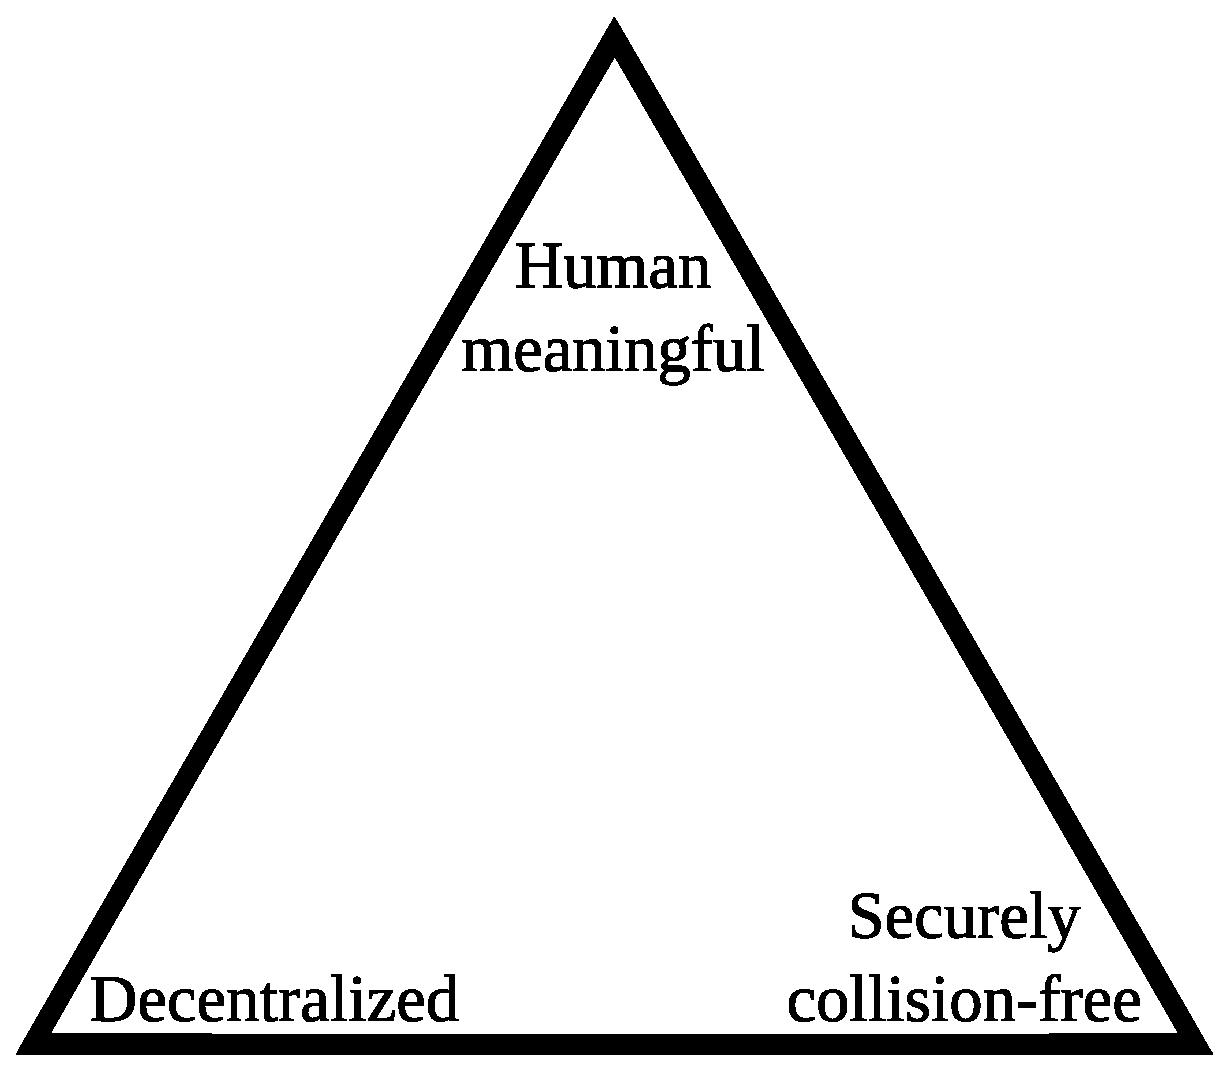
\includegraphics[width=0.3\textwidth]{images/Zooko.eps}
	\caption{Zooko's Triangle.}
	\label{fig:figure8}
\end{figure}

Tor hidden service .onion domains, PGP keys, and Bitcoin addresses are secure and decentralized but are not human-meaningful; they use the large key-space and the collision-free properties of secure digest algorithms to ensure uniqueness, so no centralized database is needed to provide this property. Tradition domain names on the Clearnet are memorable and provably collision-free, but use a hierarchical structure and central authorities under the jurisdiction of ICANN. Finally, human names and nicknames are meaningful and distributed, but not securely collision-free.\cite{Stiegler2005}

\section{Communication}



\section{Fault Tolerance}